\section{Evaluation}
\label{sec:eva}
Existing work on Linked Data query processing performs source ranking
without further optimization. We implement this source ranking
strategy to select sources first, and then use the dynamic programming
solution as proposed for Linked Data query optimization to optimize
the subsequent process. That is, the proposed query plan as well as
the operator sharing mechanism are employed to optimize cost. This is
to obtain a best-effort baseline, based on which we aim the study of
effect of the holistic treatment of source selection and query
processing, and the multi-objective optimization we propose. The
experiment shows that as opposed to our approach, the baseline yields
only a small fraction of the complete set of Pareto-optimal plans, and
the resulting suboptimal plans lead to much higher cost when producing
the same number of results.

%The evaluation of our approach consists of two parts. In the first, we
%evalute the benefit of using the dynamic programming query
%optimization algorithm for Linked Data query processing in a
%single-objective scenario. In the second part, we focus on the
%multi-objective optimization approach proposed in this paper.

% \subsection{Single-objective Optimization with Dynamic Programming}

% \subsubsection{Systems}


% \subsubsection{Results}



% \begin{figure}[htb]
%   \centering
%   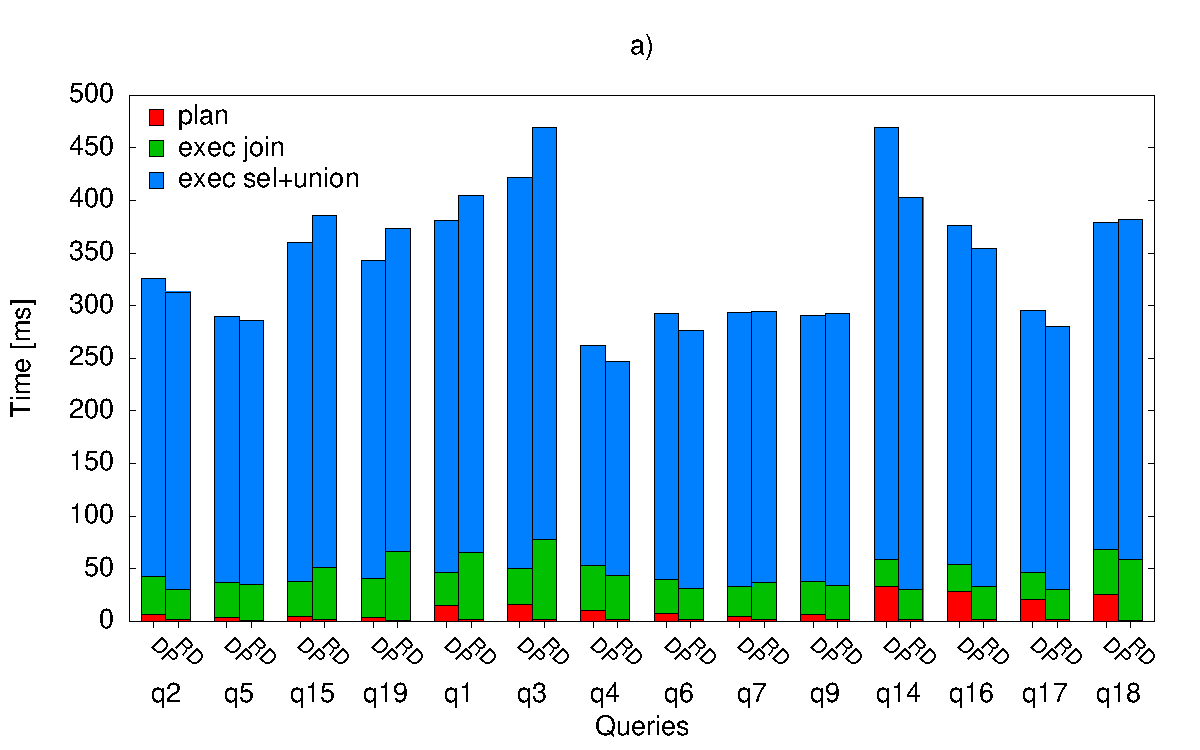
\includegraphics[width=\linewidth]{figs/exec_queries.pdf}
%   \caption{Results for execution}
%   \label{fig:exec_queries}
% \end{figure}


\begin{figure*}[htb]
  \centering
  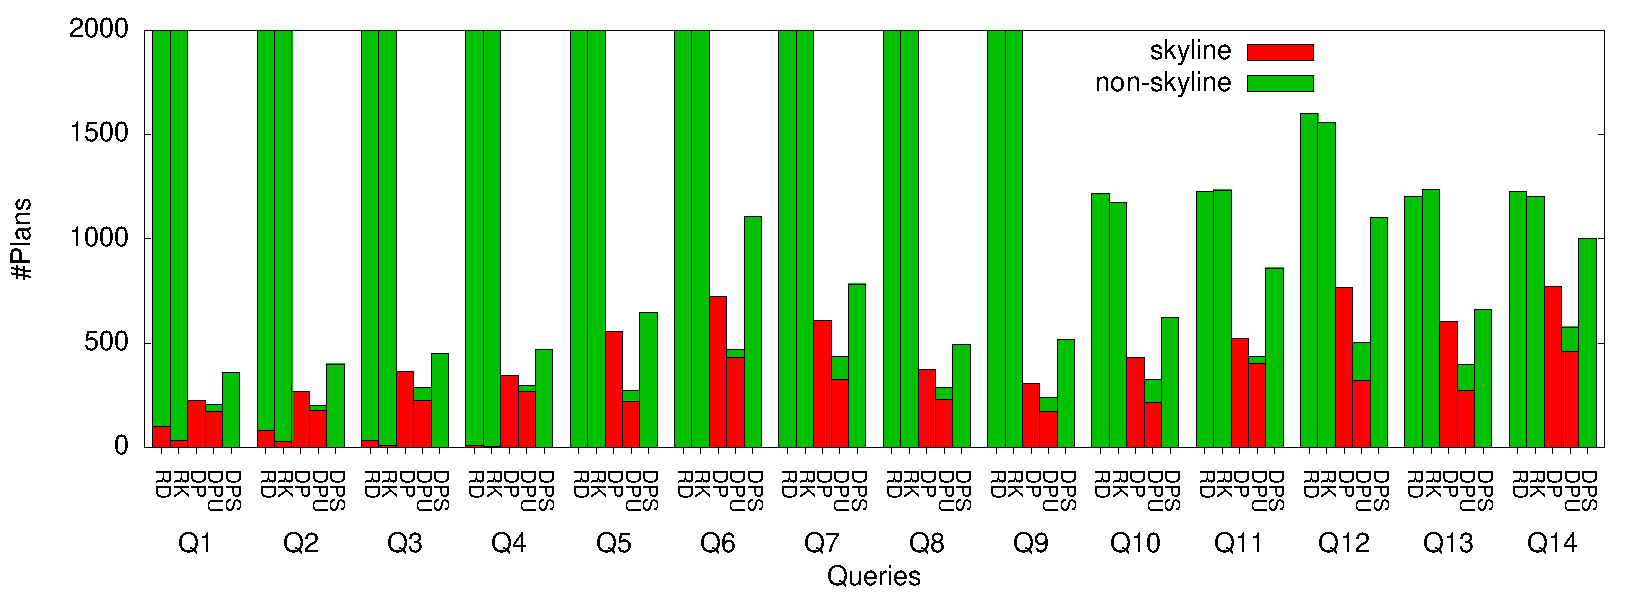
\includegraphics[width=0.7\linewidth]{figs/all_queries.pdf}
  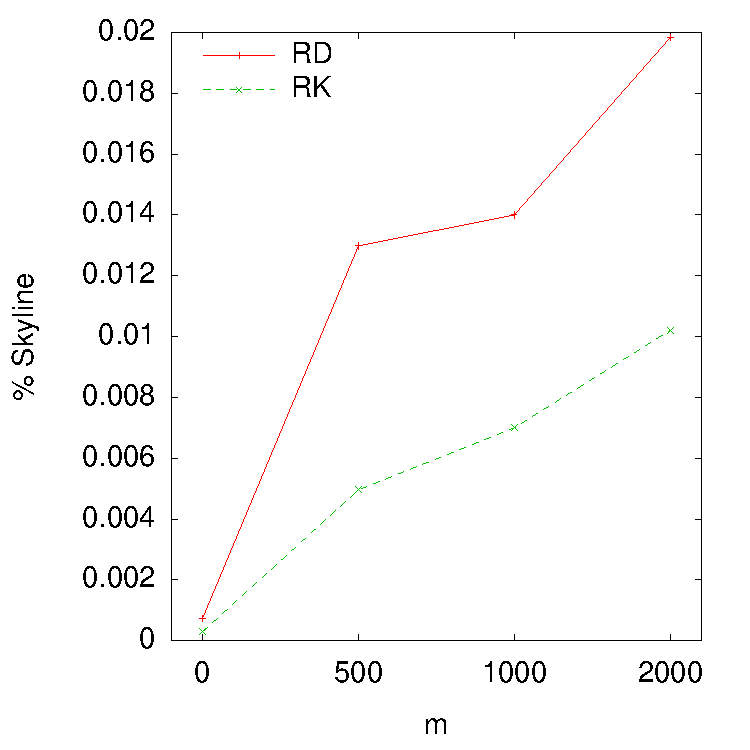
\includegraphics[width=0.29\linewidth]{figs/plans_skyline_by_m.pdf}
  \caption{a) Number of skyline and non-skyline plans for all queries
    and systems ($b=0.8, m=2000$), b) Skyline fraction for RD, RK for
    different value of $m$ ($b=0.8$).}
  \label{fig:queries}
\end{figure*}

\subsection{Systems}
\textbf{Our Approach.} We implemented three versions of our
approach. The first version (DP) implements all the proposed
techniques to produce the complete set of Pareto-optimal plans. The
second version (DPU) also uses operator sharing such that for
subsequent source accesses, the refined cost model applies. However,
the effect of this is not taken into account during pruning.  That is,
it uses directly the cost instead of the lower and upper bounds that
have been established to guarantee monotonicity of cost. Thus, at the
cost of compromising Pareto-optimality, DPU can prune more
aggressively and thus, is expected to exhibit better performance. With
this baseline, we aim to study the positive effect of using the
proposed bounds on Pareto-optimality, and to find out whether the
proposed technique for estimating the bounds is effective in reducing
the overhead resulting from that. The third version (DPS) does not use
operator sharing at all, i.e., if a source is used for more than one
triple pattern it is retrieved multiple times. We use DPS to show that
operator sharing in general is beneficial.


\textbf{Baselines.} Existing Linked Data approaches implement ad-hoc
source ranking to select few best
sources~\cite{harth_data_2010,ladwig_linked_2010}, and then process
these sources without further optimization. This processing represents
one single plan, whose optimality is unknown. We implement this source
ranking (RK) and a random source selection strategy (RD). Given the
selected sources, the standard DP solution is applied on top to
optimize the cost these baselines need to produce results from these
sources. In the same way proposed for our approach, this DP solution
applies operator sharing so that sources can be reused. Instead of one
single cost-optimized plan, our approach however yields a Pareto-set
of query plans that represents the trade-off between cost and
cardinality. Thus, we further extend these baselines to use different
combinations of sources that yield different plans.

Both baselines first retrieve all relevant sources $D$ for a query $Q$
from the source index, i.e., $D = \bigcup_{t \in Q} source(t)$. Then,
a set $\mathcal{D}$ containing $|D|$ different subsets of $D$, each
with size in the range $[1,|D|]$ is created.
%The number of  captured by and $|\mathcal{D}| = |D|$. 
The baselines differ in how these
subsets are selected:
\begin{itemize}
\item Baseline RD randomly selects the $|D|$ subsets.
\item Baseline RK first ranks sources in $D$ by the number of
  contained triples that match query triple patterns, calculated as
  $score(d) = \sum_{t \in q} card_d(t)$. The subsets are created
  by starting with the highest ranked source and then successively
  adding sources in the order of their rank to obtain $|D|$ subsets in
  total.
\end{itemize}
Each element in $\mathcal{D}$ is a subset of all relevant source and
represents a combination of sources. For each of the source
combinations, we create a single cost-optimized query plan. As a
result, we have a set of plans, which vary in the number of results as
well as because different combination of sources are used.
% using a standard dynamic
%programming optimizer (i.e., no multi-objective optimization). Sharing
%of source scan operators is also employed where possible.

Note that our approach not only selects sources (source scan
operators) but also for which triple patterns these sources are used
(selection operators), while the sources selected for the baselines
are used for all triple patterns. In order to obtain even more plans
that further vary in the number of results they produce, we create an
additional set of $m$ plans for each previously created plan by
randomly removing a subset of the inputs (selection operators) from
the unions at the root of their access plans.
%In particular, to create a new plan from an
%existing plan, for each union that is root of an access plan, we
%remove a random subset of its input (selection) operators. 
%If the source scan operator that is input for a removed selection operator is
%not shared it is also remove from the plan.
%Any invalid plans that are constructed in this way (e.g., all inputs of an union might have been) are discarded. 
In the end, each baseline has at most of $m \cdot |D|$ plans that vary
in terms of results (where only $|D|$ plans actually vary in terms of
cost).

These baselines optimize source selection independent from the
subsequent computation of results. While the goal of source selection
is to choose those that contribute many results, the subsequent
optimization focuses on cost. Compared to them, our approach not only
jointly optimize sources section and result computation but also,
considers cardinality and cost at the same time. Our goal is to study
the effect of this joint optimization on the Pareto-optimality of
plans. Further, we will investigate the effect of using non-optimal
plans on the result....
%While this effect is expected to be positive, the increased complexity of the planning problem also leads to additional cost. Thus, we will also investigate whether this overhead can be justified by looking at the total processing time needed for producing several fixed fraction of results.  


\textbf{Parameters.} Parameter $b$ specifies the benefit that is
assumed during query planning for sharing of source scan
operators. For example, with $b=0.8$ the planners assume that 80\% of
the source scan cost is saved, i.e., second and subsequent reads of a
source scan operator cost only 20\% of the first read.

For RD and RK, parameter $m$ describes the number of additional plans
that were generated by randomly remove selection and source scan
operators.

\subsection{Datasets and Queries}

We created 14 BGP queries of different sizes w.r.t. to the number of
triple patterns. We executed all queries using a link traversal
approach and recorded all retrieved sources. This dataset was then
indexed in a source index and used for the evaluation. The dataset
consists of 1,909,109 triples and contains data from various popular
open datasets, such as DBpedia, Freebase, New York Times, GeoNames,
LinkedMDB and others. Table~\ref{tab:queries} shows various
statistics for all evaluation queries.

As the source index contained too many sources for the multi-objective
optimization approach to deal with, we randomly aggregated sources
during the creation of access plans into a set of $k=5$ virtual
sources. The size of the virtual sources follows a Zipf distribution
with exponent $2$.

\begin{table}[htb]
  \centering
  \begin{tabular}{l|c|c|r}
    Query & \#Pat. & Shared [kT] & \#Res. \\%& Join-Sel. SD \\ 
    \hline

    Q2  & 3 & 1,393 & 24  \\%& 3.26\textsc{e}-5 \\
    Q5  & 3 & 1,425 & 13  \\%& 4.95\textsc{e}-5 \\
    Q15 & 3 & 1,401 & 11  \\%& 2.59\textsc{e}-5 \\
    Q19 & 3 & 1,434 & 836 \\%& 4.36\textsc{e}-5 \\
    \hline
    Q1  & 4 & 1,426 & 2   \\%& 1.30\textsc{e}-3 \\
    Q3  & 4 & 1,892 & 3   \\%& 1.89\textsc{e}-5 \\
    Q4  & 4 & 1,415 & 60  \\%& 9.58\textsc{e}-3 \\
    Q6  & 4 & 2,081 & 6   \\%& 2.62\textsc{e}-3 \\
    Q7  & 4 & 1,369 & 106 \\%& 2.75\textsc{e}-3 \\
    \hline
    Q9  & 5 & 1,405 & 17  \\%& 5.26\textsc{e}-3 \\
    Q14 & 5 & 1,830 & 20  \\%& 3.71\textsc{e}-3 \\
    Q16 & 5 & 2,396 & 1   \\%& 2.10\textsc{e}-3 \\
    Q17 & 5 & 1,409 & 1   \\%& 8.92\textsc{e}-3 \\
    Q18 & 5 & 1,007 & 2   \\%& 1.21\textsc{e}-4 \\
  \end{tabular}
  \caption{Query statistics: query name, number of patterns, number of
    triples (in thousands) contained in shared sources, number of results.}
  \label{tab:queries}
\end{table}

% \begin{table*}[htb]
%   \centering
%   \begin{tabular}{l|r|r|r|r|r|r|r|r|r|r|r|r|r|r|r|r}
%  & RD & RK & DP & DPU & RD & RK & DP & DPU & RD & RK & DP & DPU & RD & RK & DP & DPU \\
%     \hline               
                                                                                                               
%  & \multicolumn{4}{c}{Q2} & \multicolumn{4}{|c|}{Q5} & \multicolumn{4}{c}{Q15} & \multicolumn{4}{|c}{Q19}  \\

%     \hline                                                                                                   

%     \#Plans   & 1702 & 1853 & 673   & 619  & 1382 & 1871 & 446   & 446   & 2376 & 3263 & 634   & 634   & 3817 & 3240 & 761   & 761   \\
%     \#Skyline & 153  & 155  & 673   & 575  & 106  & 176  & 446   & 446   & 13   & 40   & 634   & 634   & 41   & 46   & 761   & 761   \\ 
%     \%Skyline & 22.7 & 23.0 & 100.0 & 85.4 & 23.8 & 39.5 & 100.0 & 100.0 & 2.1  & 6.3  & 100.0 & 100.0 & 5.4  & 6.0  & 100.0 & 100.0 \\
%     Time [s]  & 1.06 & 0.92 & 1.14  & 0.62 & 0.78 & 1.03 & 0.75  & 0.53  & 1.05 & 1.14 & 1.21  & 0.64  & 1.07 & 1.05 & 1.58  & 0.77  \\
  
%     \hline
%     \hline

%  & \multicolumn{4}{c}{Q1} & \multicolumn{4}{|c|}{Q3} & \multicolumn{4}{c|}{Q4} & \multicolumn{4}{c}{Q6} \\

%     \hline

%     \#Plans   & 3945 & 5362 & 866   & 832  & 4571 & 5153 & 901   & 847  & 1471 & 1306 & 453   & 465  & 954  & 1340 & 354   & 318  \\
%     \#Skyline & 0    & 0    & 866   & 689  & 0    & 0    & 901   & 699  & 1    & 0    & 453   & 434  & 0    & 1    & 354   & 283  \\ 
%     \%Skyline & 0.0  & 0.0  & 100.0 & 79.6 & 0.0  & 0.0  & 100.0 & 77.6 & 0.2  & 0.0  & 100.0 & 95.8 & 0.0  & 0.2  & 100.0 & 79.9 \\
%     Time [s]  & 1.53 & 1.67 & 7.64  & 1.60 & 1.53 & 1.62 & 10.05 & 1.80 & 1.61 & 1.29 & 1.37  & 0.75 & 1.14 & 1.33 & 1.35  & 0.70 \\

%     \hline
%     \hline

%  & \multicolumn{4}{c}{Q7} & \multicolumn{4}{|c|}{Q9} & \multicolumn{4}{c|}{Q14} & \multicolumn{4}{c}{Q16} \\

%     \hline

%     \#Plans   & 2566 & 3913 & 1035  & 813  & 2622 & 3450 & 689   & 655  & 429  & 436  & 284   & 281  & 1485 & 2265 & 685   & 663  \\
%     \#Skyline & 1    & 0    & 1035  & 781  & 0    & 0    & 689   & 637  & 0    & 0    & 284   & 281  & 0    & 0    & 685   & 583  \\ 
%     \%Skyline & 0.1  & 0.0  & 100.0 & 75.5 & 0.0  & 0.0  & 100.0 & 92.5 & 0.0  & 0.0  & 100.0 & 98.9 & 0.0  & 0.0  & 100.0 & 85.1 \\
%     Time [s]  & 1.91 & 1.50 & 20.88 & 2.28 & 1.80 & 1.64 & 23.64 & 2.56 & 1.33 & 1.21 & 0.91  & 0.41 & 1.82 & 1.99 & 14.31 & 2.38 \\

%     \hline
%     \hline

%  & \multicolumn{4}{c}{Q17} & \multicolumn{4}{|c|}{Q18} & \multicolumn{8}{c}{} \\

%     \hline

%     \#Plans   & 837  & 1022 & 398   & 286   & 1021 & 1192 & 633   & 633   & \multicolumn{8}{c}{} \\
%     \#Skyline & 1    & 0    & 398   & 286   & 0    & 0    & 633   & 633   & \multicolumn{8}{c}{} \\ 
%     \%Skyline & 0.2  & 0.0  & 100.0 & 100.0 & 0.0  & 0.0  & 100.0 & 100.0 & \multicolumn{8}{c}{} \\
%     Time [ms] & 1.67 & 1.70 & 2.68  & 0.66  & 1.53 & 1.58 & 4.15  & 1.35  & \multicolumn{8}{c}{} \\

%   \end{tabular}
%   \caption{Results for all queries, with $m=2000$ and $b=0.8$ for RD and RK.}
%   \label{tab:res}
% \end{table*}

\subsection{Setting}
All systems were implemented in Java. The query planner is
single-threaded, whereas the execution engine uses multiple
threads. All experiments were executed on a 2009 Macbook Pro with a
2.4 GHz Intel Core 2 Duo processor, 4GB RAM (of which 1GB was assigned
to the Java VM) and a Crucial m4 128GB solid-state disk.


\subsection{Results}

\textbf{Overall.} Fig.~\ref{fig:queries}a shows an overview over all
evaluation queries and displays the number of plans that were
generated by each system, split into skyline and non-skyline (i.e.,
dominated) plans. The number of skyline plans was determined by
collecting all plans of a particular query for all systems in one set
and then pruning all dominated plans. 

We can see that DP produces only skyline plans and that there are many
DPU plans that are part of the skyline (56\% on average). However, the
RD and RD baselines generate almost no skyline plans (1.9\% and 1\% on
average). DPS does not find any skyline plans.

Fig.~\ref{fig:queries}b shows the skyline fraction (i.e., the fraction
of the DP skyline) found by RD and RK for different values of $m$. We
see that for larger values of $m$ the skyline fraction is higher,
i.e., the larger plan space created by randomly removing union inputs
is necessary to find skyline plans.

\textbf{Effect of Query Size.} Figs.~\ref{fig:pareto_tp}a+b show the
planning time and found skyline fraction for different query sizes
(i.e., number of triple patterns). An increased number of triple
patterns results in a larger search space for the query optimizer: for
all systems planning time increases with the number of triple
patterns. However, the DP algorithm is much more affected than DPU,
DPS, RK and RD. Going from 3 to 5 triple patterns, the planning time
of DP increases by a factor of 101.4, DPS increases by a factor of 28,
while the planning time for DPU only increases by a factor of 18, and
RD and RK are largely unaffected. The high increase in planning time
for 5 triple patterns is largely due to query Q16. Without Q16, the
factors decrease to 60.7, 11.2 and 14 for DP, DPU and DPS,
respectively.

The better performance of DPU than DPS indicates that DPU is able to
prune more plans, because operator sharing can produce better
plans. This also supported by the fact that DPS on average creates
more plans than either DP or DPU (see
Fig.~\ref{fig:queries}a). Compared to DPU, DP is not able to prune as
many intermediary plans because of the estimated bounds that allow
pruning only when there is no possibility that a plan might be part of
an optimal plan.

% dp 71282
% dpu 5128
% dps 17024

Fig.~\ref{fig:pareto_tp}b shows the fractions of the complete plan
skyline (i.e., the plans computed by DP) that the systems are able to
calculate for different query sizes. Whereas for 3 triple patterns the
baselines RD and RK are able to find 11\% and 6\% of the skyline, no
skyline plans are found for 4 and 5 triple patterns. DPU also performs
better for 3 triple patterns, where 70\% of the skyline is found (54\%
for 4 and 5 triple patterns). For more triple patterns the space of
possible plans is much larger, which is why especially the baselines
perform much worse.

\begin{figure}[htb]
  \centering
  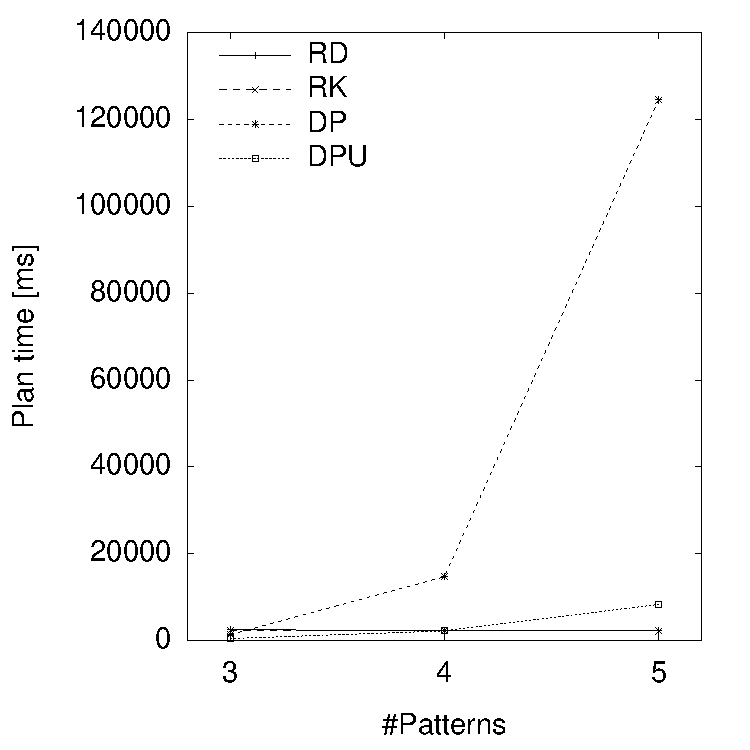
\includegraphics[width=0.49\linewidth]{figs/pareto_plan_tp.pdf}
  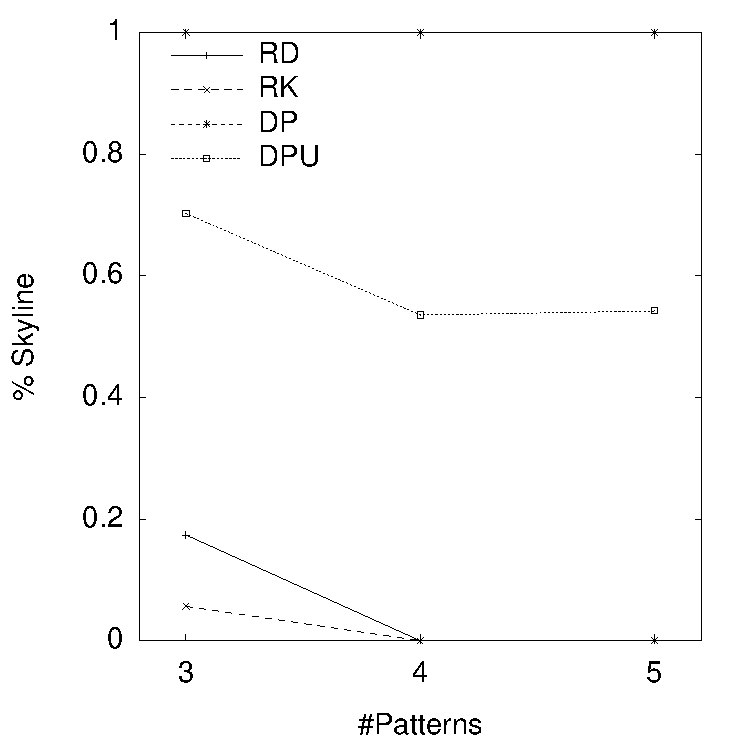
\includegraphics[width=0.49\linewidth]{figs/plans_skyline_by_tp.pdf}
  \caption{Effect of query size on a) planning time and b) skyline
    fractions ($b=0.8, m=2000$).}
  \label{fig:pareto_tp}
\end{figure}

\textbf{Effect of Sharing Benefit.} Figs.~\ref{fig:pareto_sharing}a+b
show the planning time and skyline fractions for different values of
the sharing benefit $b$. We see in Fig.~\ref{fig:pareto_sharing}a that
the planning times for DPS, RD and RK are not affected by different
values for $b$, which is expected as these planners do not take the
sharing benefit into account.

However, for DP the planning time increases with higher sharing
benefits: from 36.7s for $b=0.1$ to 47.7s for $b=0.8$.  The planning
time for DP increases with higher sharing benefits because the bounds
of plan costs are less tight and less plans can be pruned during the
query optimization process. DPU on the other shows the opposite
behavior, planning time decreases from 13.2s ($b=0.1$) to 3.8s
($b=0.8$). Again, DPU is able to prune more plans when the expected
sharing benefits are higher as this creates a steeper cost gradient
between plans.

Fig.~\ref{fig:pareto_sharing}b shows the skyline fractions for all
approaches for different values of $b$. We can see that DPU computes a
larger part of the skyline when the sharing benefit is lower. This is
due to the fact that DPU does not take the effect of operating sharing
into account, leading to worse results the more pronounced the
influence of the sharing benefit is. The other approaches, DPS, RD and
RK, are not affected by the sharing benefit as the benefit is not
taken into account during planning.

\begin{figure}[htb]
  \centering
  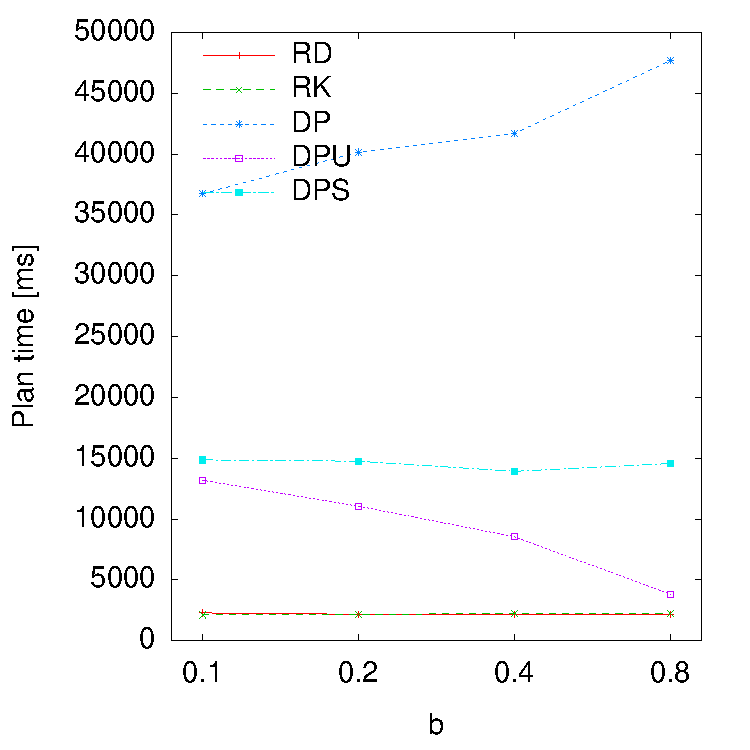
\includegraphics[width=0.49\linewidth]{figs/pareto_plan_b.pdf}
  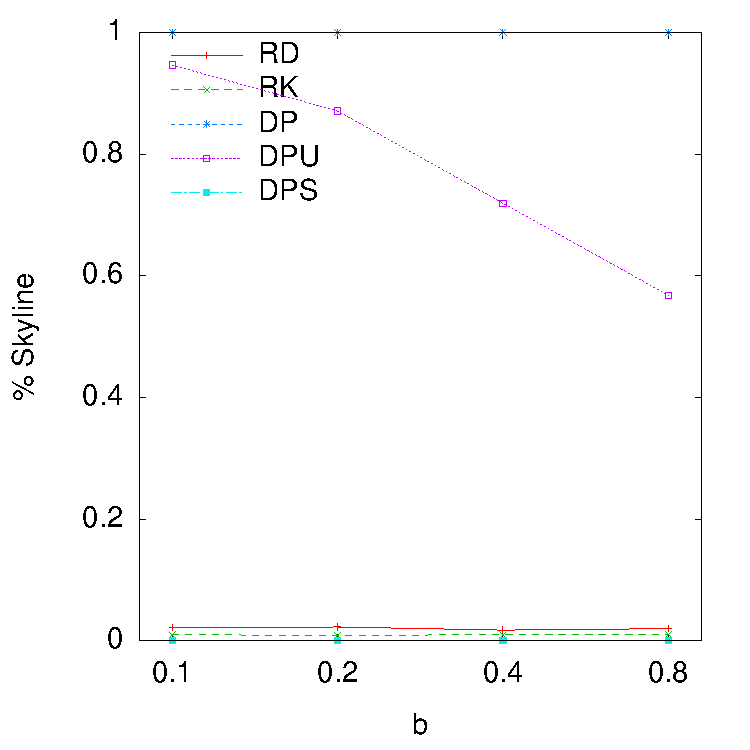
\includegraphics[width=0.49\linewidth]{figs/plans_skyline_by_b.pdf}
  \caption{Effect of sharing benefit on a) planning time and b)
    skyline fractions ($m=2000$).}
  \label{fig:pareto_sharing}
\end{figure}

\textbf{Plan Skyline.} Figs.~\ref{fig:pareto_q2_skyline}a+b show a
scatter plot of cost and cardinality of plans generated by all systems
for query Q2. In these plots a plan dominates all plans that are to
its lower right, i.e. that have higher cost (x-axis) and lower
cardinality (y-axis). Fig.~\ref{fig:pareto_q2_skyline}a shows all
plans that were generated by the different systems. We can immediately
see that many of the plans generated by the RD and RK baselines are
dominated by other plans and that all DPS plans are also
dominated. Fig.~\ref{fig:pareto_q2_skyline}b shows only the plans for
all systems that are on the skyline. Here, the dominated DPS plans no
longer appear and only few RD and RK plans remain.

\begin{figure}[htb]
  \centering
  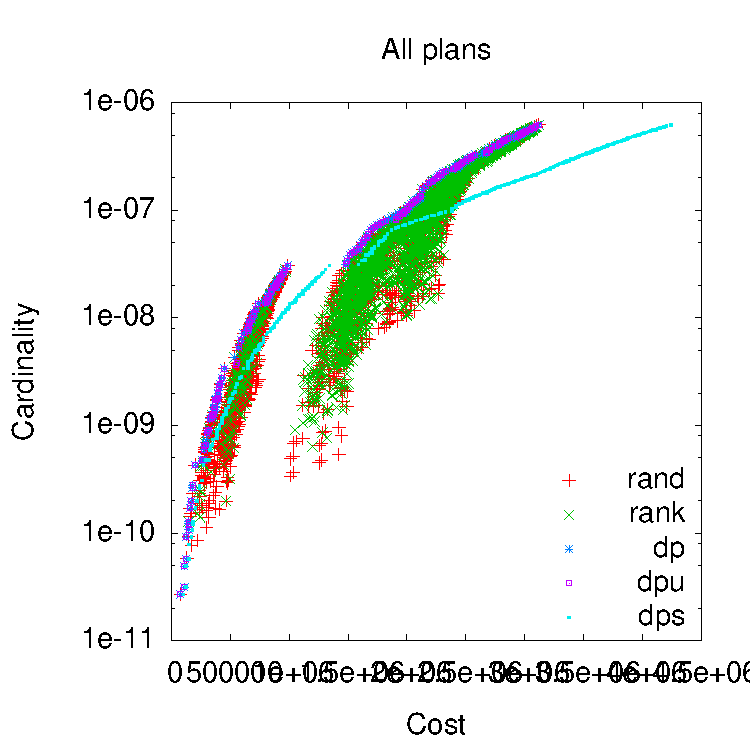
\includegraphics[width=0.49\linewidth]{figs/plans_q2_all.pdf}
  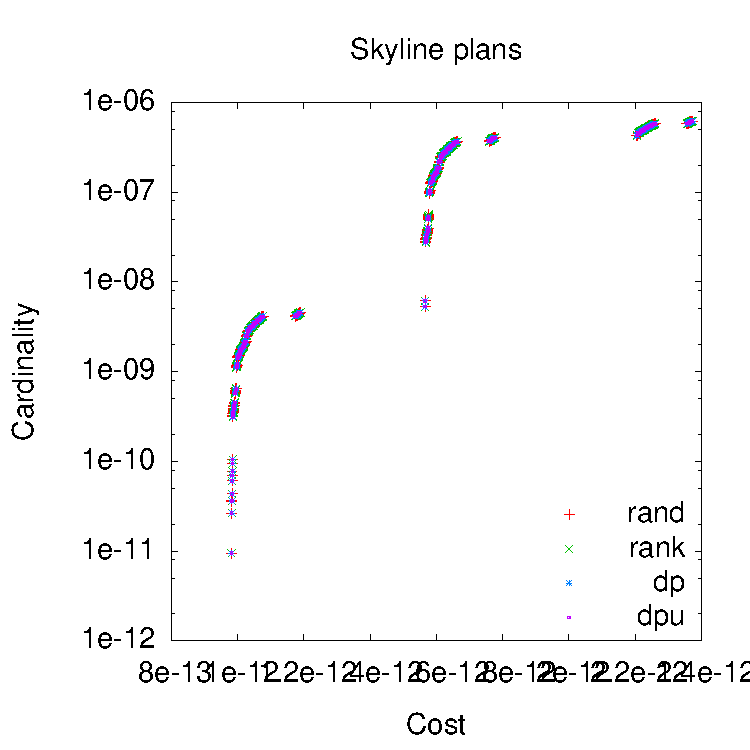
\includegraphics[width=0.49\linewidth]{figs/plans_q2_sky.pdf}
  \caption{Plans for query Q2 on all systems: a) all plans and b)
    skyline plans ($b=0.8,m=2000$).}
  \label{fig:pareto_q2_skyline}
\end{figure}

\textbf{Execution Time.} We selected three queries with different
result set sizes (Q2: 24, Q7: 106, Q9: 836) and randomly chose 20\% of
the plans generated by each system in order to execute them an record
the over all query time (planning and execution). Fig.~\ref{fig:exec}
shows the averaged results for all three queries. Each point in a
graph is the average execution time of all plans that produce a
particular number of results. For example, all DPU plans for query Q7
that produce 46 results on average had an total query time of
7.3s. Tab.~\ref{tab:exectimes} shows the average total query times for
all systems for all three queries.

% sqlite> select system,avg(t_plan+t_execute) from runs where b=0.8 and query='q2' and delay=0 group by system;
% dp|15810.3125
% dps|24779.7794117647
% dpu|15532.1785714286
% rand|4450.47596153846
% rank|18929.3333333333

% sqlite> select system,avg(t_plan+t_execute) from runs where b=0.8 and query='q7' and delay=0 group by system;      
% dp|29751.0277777778
% dps|75013.9090909091
% dpu|16421.2794117647
% rand|21933.95
% rank|23302.0

% sqlite> select system,avg(t_plan+t_execute) from runs where b=0.8 and query='q19' and delay=0 group by system;     
% dp|18151.0384615385
% dps|31050.8214285714
% dpu|16669.8846153846
% rand|18244.5434782609
% rank|21884.4935897436

% sqlite> select query,system,avg(t_plan+t_execute) from runs where b=0.8 and query in ('q2', 'q7', 'q19') and delay=1500 group by query,system order by query;                                                                        
% q19|dp|22841.4871794872
% q19|dps|35001.9166666667
% q19|dpu|20911.262195122
% q19|rand|23130.6666666667
% q19|rank|26869.314516129
% q2|dp|20703.0909090909
% q2|dps|29921.3793103448
% q2|dpu|21166.1097560976
% q2|rand|23554.1111111111
% q2|rank|25453.0075757576
% q7|dp|36376.4537037037
% q7|dps|97149.75
% q7|dpu|30350.3928571429
% q7|rand|27545.1532258065
% q7|rank|27654.7661290323

\begin{table}[htb]
  \centering
  \begin{tabular}{l|r|r|r|r|r}
        & DP   & DPU  & DPS  & RD   & RK   \\
    \hline
    Q2  & 15.8 & 15.5 & 24.8 & 4.5  & 19.9 \\
    Q7  & 29.8 & 16.4 & 75.0 & 21.9 & 23.3 \\
    Q19 & 18.2 & 16.7 & 31.1 & 18.2 & 21.9 \\
  \end{tabular}
  \caption{Average total query times (in seconds) for all plans of queries Q2, Q7, Q19.}
  \label{tab:exectimes}
\end{table}

For Q2, the average total time of RD is much lower than the other
systems, but from Fig.~\ref{fig:exec} we see that none of the sampled
plans produces more than 7 results, leading to the much lower
average. On the other hand, DP and DPU, as well as RK, calculate all
results, but DPU and DPU outperform RK in terms of the total average
by \~22\%. When not producing all results, the gains are higher: for
example, to produce 7 results, DP requires only 35\% of the time that
plans for RK need. The lack of operator sharing leads to much worse
performance for DPS, especially when more results are reported.

While DPU is able to outperform the baselines RK and RD for query Q7,
the larger overhead of DP leads to a worse total average for all
result sizes. The benefit of DPU is more pronounced for plans that
produce fewer results, for 28 results DPU requires only 28\% of the
time that plans for RK and RD need.

The situation is similar for query Q19. Here, on average DPU is better
than DP, RD and RK, whereas DP and RD have the same average. However,
both DPU and DP perform better than the baselines when only partial
results are reported. Plans for DP and DPU that report 205 results on
average require only 35\% of the processing time than RK plans for the
same number of results.

% First, we see that the RD baseline does not always find plans that
% produce all results (Q2, Q19), whereas RK is able to produce all
% results as RK prefers sources that contain many triples matching query
% triple patterns. DPS overall has the worst execution time, showing the
% large benefit of operator sharing. For queries Q2 and Q10 plans of DP
% and DPU generall perform better than the baselines, especially when
% only partial results are reported. For Q7, only DPU performs better
% whereas here the higher overhead leads to worse performance for DPU.

% Fig.~\ref{fig:exec_q7} shows the execution
% times and number of results for 20\% of plans (randomly chosen) for
% queries Q2, Q7 and Q19 for all approaches. 

% We see that plans that produce less results
% in general have shorter execution times. In order to find all 106
% query results, the fastest plan takes 17.9 seconds; producing a subset
% of 46 results requires only 4.3 seconds.

However, we can also see that some of the plans produce no results at
all. This is due to the fact that the employed cardinality estimation
procedure does not take dependencies between sources into
account. Here, a more sophisticated method for cardinality estimation
would help avoid generating empty plans.

\begin{figure*}[htb]
  \centering
  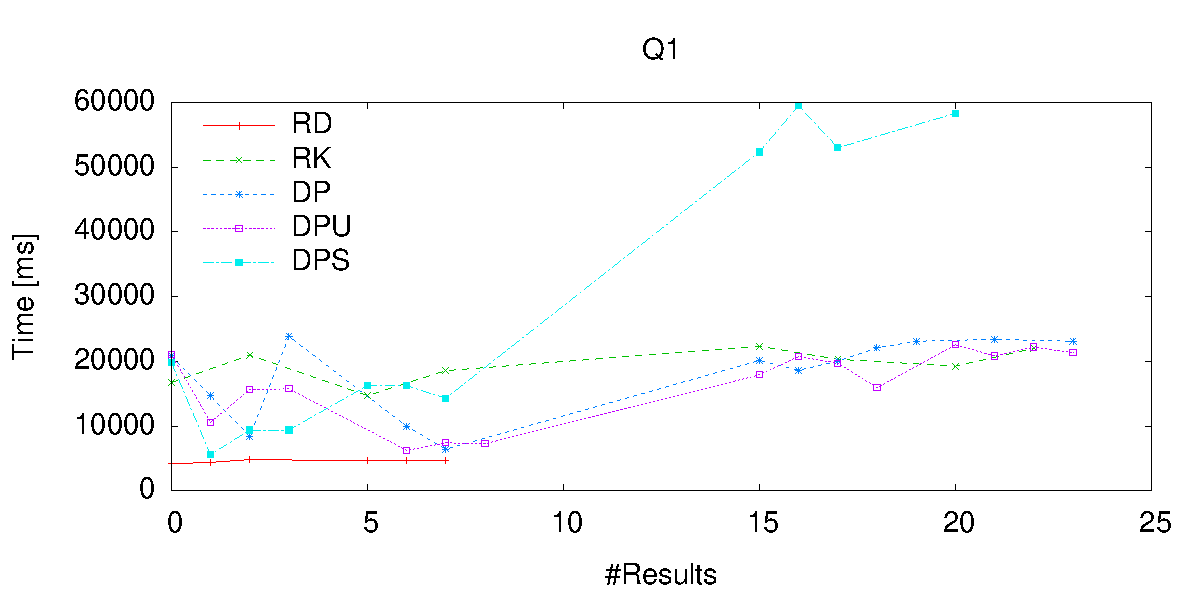
\includegraphics[width=0.32\linewidth]{figs/pareto_exec_0_q2.pdf}
  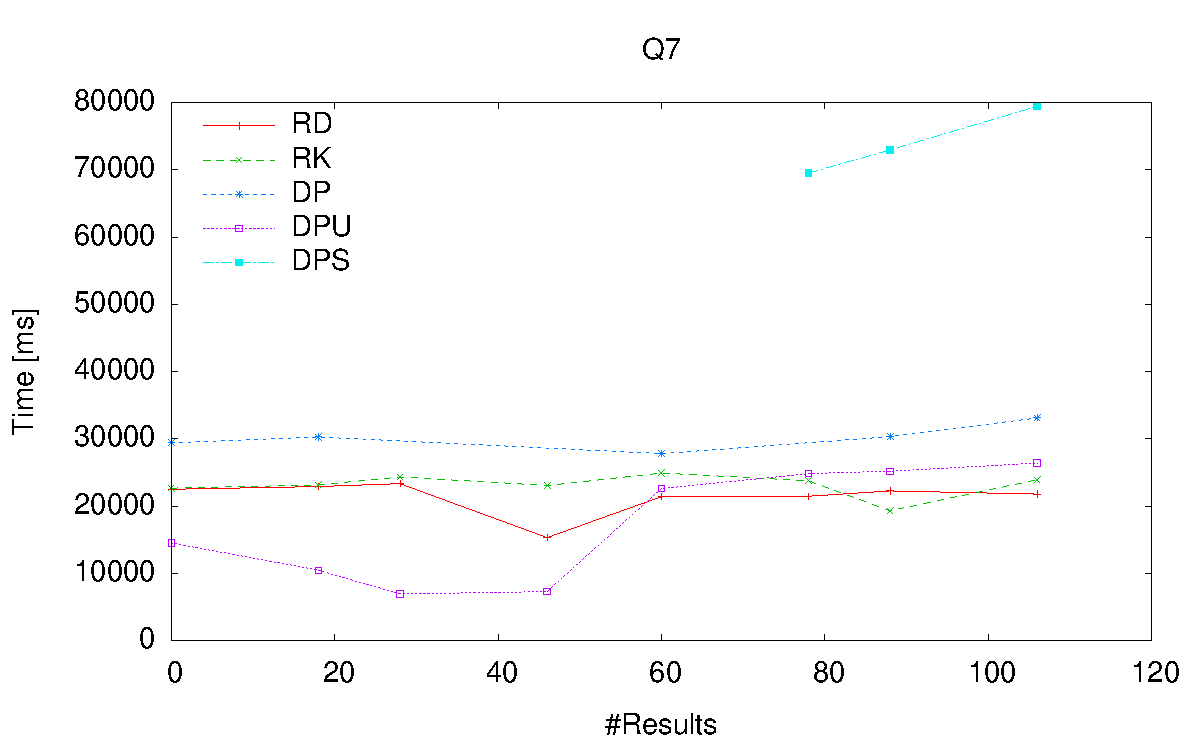
\includegraphics[width=0.32\linewidth]{figs/pareto_exec_0_q7.pdf}
  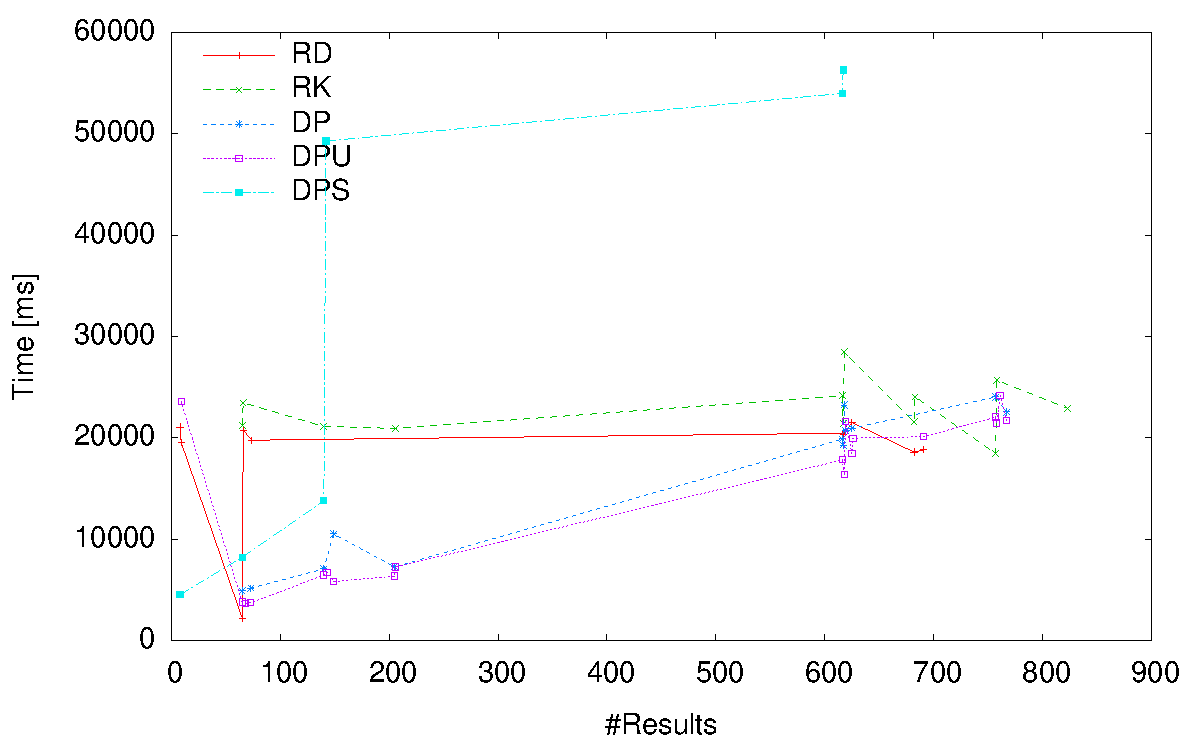
\includegraphics[width=0.32\linewidth]{figs/pareto_exec_0_q19.pdf}
  \caption{Execution times of query plans for queries Q2, Q7 and Q19.}
  \label{fig:exec}
\end{figure*}
%%% Local Variables: 
%%% mode: latex
%%% TeX-master: "paper"
%%% End: 
